\chapter{METHODOLOGY}
In this chapter, the methodology is detailed as follows. 
First, we describe the architecture of the model. 
Second, we explain all pre-training loss functions used in this experiment.
Third, the details of \acrshort{pos} tagging are provided. 
Fourth, we outline the datasets used in this experiment. 
Lastly, we provide details on the visual question answering setup.

\begin{figure}[h]
    \caption{Overall methodology}
    \label{fig:overview}
    Pre-training the model with a \acrshort{mlm} task by masking tokens based on the \acrshort{pos} in the image captions.
    \begin{center}
        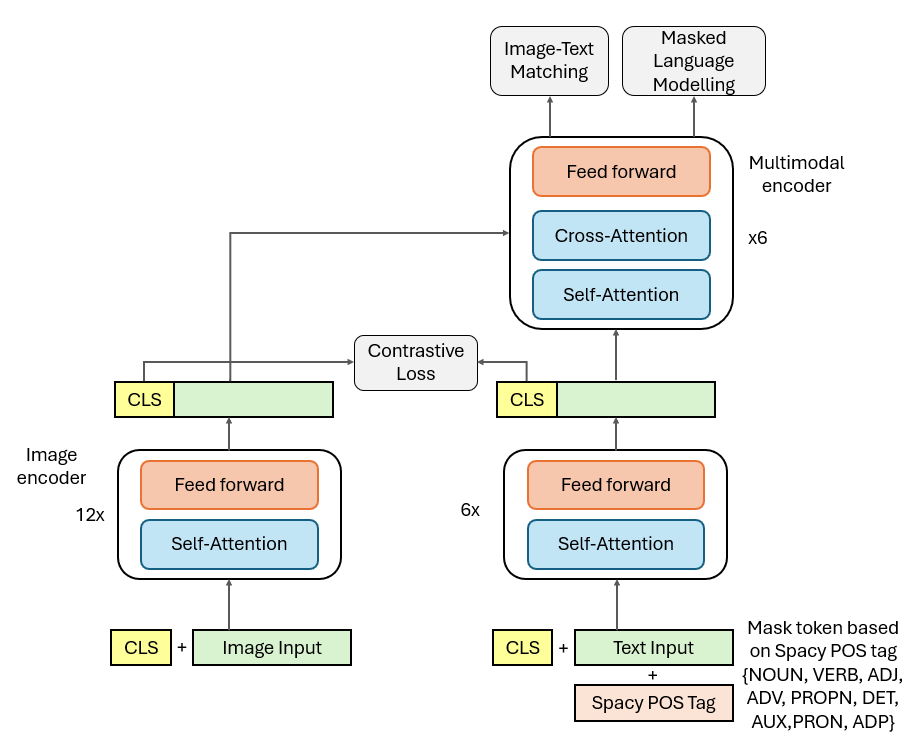
\includegraphics[width=0.8\textwidth]{Images/overview.png}
    \end{center}
    \small
\end{figure}

\section{Model architecture}
As shown in Figure \ref{fig:overview}, our model includes three main components: an image encoder, a text encoder, and a multimodal encoder. 
The first component is the image encoder, for which we use ViT \cite{vit}, modified following \cite{clip}, as the image encoder in this experiment. 
The second component is the text encoder, which employs a transformer architecture as BERT \cite{bert} to encode image captions with BERT tokenizer for tokenization.
The final component is the multimodal encoder, where \acrshort{vl} interactions occur.

Given a training dataset \(D\) consisting of image-text pairs \((I_i, T_i) \in D\), where \(I_i\) is the image and \(T_i\) is the image caption of the \(i\)-th image, each image is first encoded as a sequence of tokens \(\{v_{cls}, v_1, \dots, v_n\}\) using ViT \cite{vit}. 
Here, \(v_{cls}\) represents the embedding of the [CLS] token prepended to the image patch sequence. 
In this experiment, the image encoder was initialized with ViT-B-32 pre-trained on ImageNet-21K \cite{imagenet}.
Next, we use a 6-layer transformer, randomly initialized, to encode the image caption \(T_i\) into text embeddings \(\{w_{cls}, w_1, \dots, w_n\}\), where \(w_{cls}\) is the embedding of the [CLS] token. 
Finally, both text and image encodings are passed through the multimodal encoder to fuse both inputs, producing multimodal encodings. 
For the multimodal encoder, a cross-attention layer is used, where both keys and values are the image encodings, and the text encoding serves as the query in the cross-attention layer.


% Cross Attention using Image = K, V Text as a query.
% Thought: The image encoder choice can be change based on training speec.
\section{Pre-training objectives}
In this work, we pre-train our model with three objectives: \acrfull{mlm}, \acrfull{itc} and \acrfull{itm}.
\subsection{Mask language modelling}
Our model is trained with the \acrlong{mlm} task. 
Typically, a percentage of tokens \(\{w_1, \dots, w_T\}\) are replaced with a special [MASK] token to create a masked caption \(T^{\text{mask}}\). 
However, in this work, the masked tokens are selected based on \acrshort{pos} type instead of randomly masking. 
The model is then trained to predict the original tokens at the masked positions, conditioned on both the unmasked tokens in \(T^{\text{mask}}\) and the visual features of \(I\) as \(p^{\text{mask}}(I, T^{\text{mask}})\).
Let \(y^{\text{mask}}\) be a one-hot vector representing the ground-truth vocabulary for the masked token, where the masked token has a probability of 1. 
The model’s objective is to minimize the cross-entropy \(\mathbf{H}\), given by:
\[
    \mathcal{L}_{\text{MLM}} = \mathbf{H}(y^{\text{mask}}, p^{\text{mask}}(I, T^{\text{mask}})S))
\]

\subsection{Image-text contrative learning}
To improve each unimodal encoders representation, we use \acrlong{itc} to improve alignment of each modality.
\acrshort{itc} aims to improve alignment by maximize similarity score of image and text from the same pair with score function \(s(I, T) = v_{cls}^\top w_{cls}\), and minimize similarity score of image and text not from its pair.
We then calculate softmax-normalized similiarity score for each image to any text and each text to any image, identified as image-to-text \(p^{i2t} \in \mathbb{R}^{M}\) and text-to-image \(p^{t2i} \in \mathbb{R}^{M}\) score as:
\[
    p^{i2t}_i(I) = \frac{ \exp{(s(I,T_i))/\tau} }{ \sum_{m=1}^{M}\exp{(s(I,T_m)/\tau} }, \quad p^{t2i}_i(T) = \frac{ \exp{(s(T,I_i))/\tau} }{ \sum_{m=1}^{M}\exp{(s(T,I_m)/\tau} }
\]
where \(\tau\) is a learnable temperature parameter. Let \( y^{i2t}(I) \in \{0,1\}^M \) and \( y^{t2i}(T) \in \{0,1\}^M \) be a ground truth with probability of 1 at a position of same pair, and probability of 0 on the otherhand.
The \acrshort{itc} loss is calculated as cross-entropy \(\mathbf{H}\) between \(p\) and \(y\):
\[
    \mathcal{L}_{\text{ITC}} = \frac{1}{2}(\mathbf{H}(y^{i2t},p^{i2t}) + \mathbf{H}(y^{t2i},p^{t2i}))
\]
\subsection{Image-text matching}
To further improve multimodal alignment in the \acrshort{vl} model, \acrlong{itm} is employed to enhance alignment. 
The model is trained to predict whether an image and caption are from the same pair. 
A fully connected layer, followed by a softmax function, is added over the model. 
This layer takes the [CLS] embedding from the multimodal encoding as input to predict whether the pair is positive (matched) or negative (unmatched). 

The loss function for \acrshort{itm}, using cross-entropy loss, is defined as:
\[
    \mathcal{L}_{\text{ITM}} = \mathbf{H}(y^{\text{itm}}, p^{\text{itm}}(I, T)),
\]
where \(y^{\text{itm}}\) is a one-hot ground-truth label, and \(p^{\text{itm}}(I, T)\) is the predicted class probability.

The full pre-training objective of our work can be written as:
\[
    \mathcal{L} = \mathcal{L}_{\text{MLM}} + \mathcal{L}_{\text{ITC}} + \mathcal{L}_{\text{ITM}}
\]

\section{Part of speech masking}
In this experiment, we explored the effect of each \acrshort{pos} on \acrshort{vl} learning in term of performance, efficiency and training loss.
For each image caption, each token have to be classified into \acrshort{pos} categories for masking.
We use POS-tagging tools SpaCy\footnote{POS-tagging tool SpaCy: https://spacy.io/} to classify each word into \acrshort{pos} classes based-on the Universal POS tag set\footnote{Universal POS tag set: https://universaldependencies.org/u/pos/}.

\section{Pre-training dataset}
We pre-trained the model on the Conceptual Captions dataset \cite{conceptual-caption}, which consists of 3.3 million image-text pairs. 
In Conceptual Captions dataset, an automated process was used to select, filter, and refine these image-caption pairs to ensure they are clear, informative, and suitable for effective model training.

\section{Evaluation}
In this work, we evaluate each model trained with different types of \acrshort{pos} masking through image-text retrieval and visual question answering tasks. 
Details of the evaluation methods and datasets used in these tasks are provided in this section.

\subsection{Image-text retrieval}
For the image-text retrieval task, we evaluate the effect of masking on each \acrshort{pos} category by performing zero-shot evaluations on the Flickr30K \cite{flickr30k} and VALSE \cite{valse} datasets for both image-to-text and text-to-image retrieval. 
The Flickr30K dataset is used to assess the model's overall performance in retrieval tasks. 
To gain deeper insights, we evaluate our model using the VALSE dataset, which categorizes linguistic phenomena into six distinct types: existence, plurality, counting, relation, action, and coreference.
Each image caption in the VALSE dataset also includes a "foil" version, where words related to each caption category are modified. 
This setup allows us to analyze how different \acrshort{pos} masking strategies affect the model's retrieval performance and the alignment between visual and textual representations.

\subsection{Attribution, Relation and Order benchmark}
As demonstrated by \citeA{rf-curriculum-masking}, the results suggest that masking strategies impact a model’s ability to understand attributes, relationships, and word order. 
In this work, we also benchmark each pre-trained model with specific \acrshort{pos} masking against four tasks proposed by \citeA{vl-bag-of-word}: \acrfull{vgr}, \acrfull{vga}, \acrfull{co}, and \acrfull{fo}. 
This benchmark is designed to assess the \acrshort{vl} model’s understanding of compositional relationships by swapping and replacing words in image captions, such as altering "The horse is eating the grass" to "The grass is eating the horse." 
Evaluating models against this benchmark provides valuable insights into their semantic and context understanding of vision and language modality.

\begin{figure}[h]
    \caption{Visual question answering model architecture}
    \label{fig:vqa}
    Modified model architecture for \acrshort{vqa} task.
    \begin{center}
        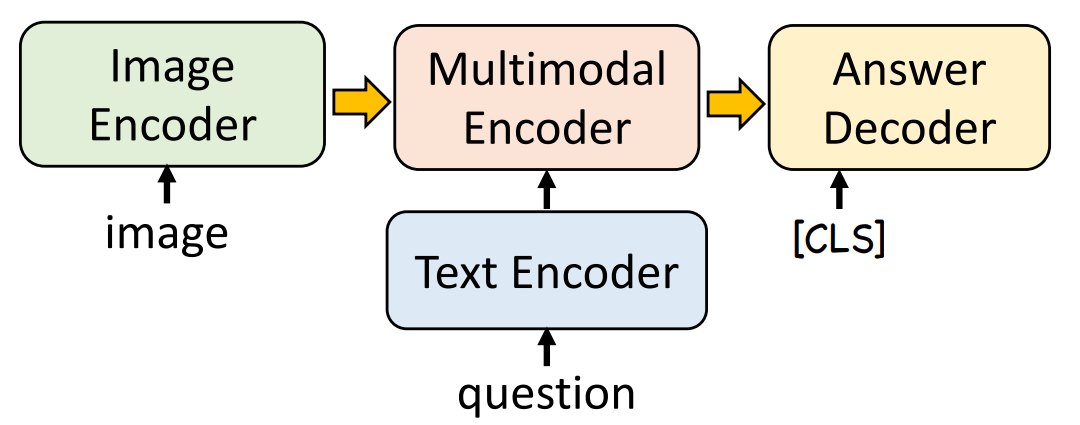
\includegraphics[width=0.6\textwidth]{Images/vqa_method.png}
    \end{center}
    \small
\end{figure}

\subsection{Visual question answering}
The \acrfull{vqa} task requires the model to generate answers, which require an additional decoder over the multimodal encoder, as shown in Figure \ref{fig:vqa}. 
In this work, we append a 6-layer transformer as a decoder, initialized with the parameters of the multimodal encoder. 
Answers are generated in an auto-regressive manner, with multimodal embeddings as input and a special start-of-sequence token ([CLS]) as the initial input to the decoder.
The benchmark dataset for the \acrshort{vqa} task is the VQA2.0 dataset \cite{vqa2}, which is constructed using images from COCO \cite{mscoco}. 
This dataset includes 83,000 images for training, 41,000 for validation, and 81,000 for testing.
We further train our model using the VQA2.0 training set.
We categorized each question into six categories following VALSE linguistic phenomena categories to provide deeper insights.
